The principle of the DP algorithm to solve the Knapsack problem is that, if the last item is rejected, the best profit will only depend on the remaining items with the full capacity of the knapsack. In contrast, if it is selected, the best profit includes the profit of this item and the best profit obtainable from the remaining items with the remaining capacity of knapsack after subtracting the weight of the last item. 

Therefore, the DP procedure is to construct a profit table with each row corresponding to an item and the number of columns depending on the knapsack capacity with unit step. The profit value of each cell will be calculated based on the current capacity, the corresponding item as well as the recursive relation with the previous cells, which can be explained as follows. At any cell corresponding to an item and a value of capacity, if the item is heavier than the available capacity, it will be rejected and the profit value of the cell is obtained from the previous items. In contrast, it is necessary to compare the profit obtainable with and without that item. The set of the previous items must ensure enough capacity if new item is selected.

\paragraph*{One-state devices}
In the context of one-state devices, each device is considered as an item with its power demand as weight, while the profit is computed from the power demand as well as the operating probability. Although the absolute error between the aggregate power and the total power demand of the identified devices is a criterion to identify the operating devices, it does not satisfy the recursive relation. Concretely,
\begin{eqnarray}
&&\left |\sum_{j=1}^i{w_js_j-x}\right | \neq w_is_i +\left |\sum_{j=1}^{i-1}{w_js_j}-x\right |\\
\mbox{if } &&w_is_i \times \left (\sum_{j=1}^{i-1}{w_js_j}-x\right )<0.\nonumber
\end{eqnarray}

To overcome this restriction, we construct two separated tables, $P^1_e$ and $P^1_l$, for the power and the probability parameters, respectively. Each table is composed of $N$ rows and $R$ columns with $R=\lceil x+\epsilon\rceil$, where $\lceil . \rceil$ is the rounding up operator. The entry of the first table $P^1_e(i,\beta)=\sum_{j=1}^i{w_js_j-x}$ and second table $P^1_l(i,\beta)=\lambda \times \sum_{j=1}^i{L^1(s_j)}$ are calculated by Algorithm~\ref{algo1}. A flag table $F$ is also constructed to mark if a device is running or not.
\begin{algorithm}
\caption{Entry calculation for profit tables in case of one-state devices.}
\label{algo1}
\begin{algorithmic}[1]
\Ensure $P^1_e(i,\beta),P^1_l(i,\beta)$
\State $a^1_1 = P^1_e(i-1,\lfloor \beta-w_i\rfloor)+w_i$
\State $a^1_2 = P^1_l(i-1,\lfloor \beta-w_i\rfloor)+\lambda \times l^1_{i1}$
\State $b^1_1 = P^1_e(i-1,\beta)$
\State $b^1_2 = P^1_l(i-1,\beta)+\lambda \times l^1_{i0}$
\State $A^1 =  \left |a^1_1\right|+a^1_2$
\State $B^1 = \left |b^1_1\right |+b^1_2$
\State $F(i,\beta) = 0$

\If{$w_i \leq \beta$ and $ A^1 \leq B^1$}
  \State $P^1_e(i,\beta) =  a^1_1$
  \State $P^1_l(i,\beta) = a^1_2$
  \State $F(i,\beta) = 1$
\Else
  \State $P^1_e(i,\beta)= b^1_1$
  \State $P^1_l(i,\beta)= b^1_2$
\EndIf
\end{algorithmic}
\end{algorithm}
In Algorithm~\ref{algo1}, because the weight of an item is not an integer number, the notation $\lfloor . \rfloor$ is used to round down the value of $(\beta-w_i)$. The values of $A^1$ and $B^1$ denote the profit obtainable with and without new device in the list of operating ones, respectively. The case that gives better profit is then selected and the respective values are filled in the tables. The initial conditions of each tables are
\begin{eqnarray*}
P^1_e(0,\beta)& =&-x,\beta = 0,\ldots, R\\
P^1_l(0,\beta)& = &0,  \beta = 0,\ldots,R\\
P^1_e(i,0)&=& -x,i=1,\ldots,N\\
P^1_l(i,0) &= &\sum_{j=1}^i{\lambda \times l^1_{j0}},i=1,\ldots,N.
\end{eqnarray*}
After calculating all entries of the profit tables, a backtracking procedure, illustrated in Algorithm~\ref{algo2}, is used to backtrack through the tables from the last cell to obtain the set of running devices with aid of the flag table $F$.

\begin{algorithm}
\caption{Backtracking algorithm in case of one-state devices.}
\label{algo2}
\begin{algorithmic}[1]
\Ensure State indicator vector $\mathbf{s} = \{s_1,\ldots,s_N\}$ 
\State $i = N$
\State $\beta =  R $
\While{$i > 0$ and $\beta>0$}
\If{$P^1_e(i,\beta) \neq P^1_e(i-1,\beta)$ or $F(i,\beta)=1$}
\State $s_i = 1$
\State $\beta = \beta-\lceil w_i \rceil $
\State $i = i-1$
\Else
\State $s_i=0$
\State $i = i-1$
\EndIf
\EndWhile
\end{algorithmic}
\end{algorithm}

Let consider an example for three devices with the respective weight and operating probability: $(w_1,p_1) = (2,0.8)$, $(w_2,p_2) = (5,0.3)$, $(w_3,p_3) = (3.5,0.9)$.
With $P = 10$, $x = 5$, $\epsilon=0.5$, the log-linear form of the operating probability of each device, i.e. $l_{i0} = -\log{(1-p_i)}$ and $l_{i1} = -\log{p_i},i = 1,\ldots,3$, are $(l_{10},l_{11})=(0.7,0.1)$, $(l_{20},l_{21})=(0.15,0.52)$, $(l_{30},l_{31})=(1,0.05)$, respectively, and the boundary of total power $R$ is equal to 6.

The entries of the profit tables are calculated by Algorithm~\ref{algo1} and filled in Table~\ref{table:DP1}. The best profit is obtained at $(i,\beta)=(N,R)$. From this optimal point, the respective combination of running devices can be determined by backtracking through the table by applying Algorithm~\ref{algo2}. As a result, $\mathbf{s} = (1,0,1)$, i.e. the first and third devices are operating while the second one is turned off. Apparently, this combination of devices gives the least absolute error on the power as well as the maximum operating probability.

\begin{table}
\caption{Running example of DP in SmartSense for one-state devices}\label{table:DP1}
\begin{center}
\begin{tabular}{|c|c|c|c|c|c|c|c|}
\hline
\multicolumn{8}{|c|}{$P^1_e(i,\beta)$}\\ \hline 
$(i,\beta)$&0&1&2&3&4&5&6\\ \hline
0&-5&-5&-5&-5&-5&-5&-5 \\ \hline
1&-5&-5&-3&-3&-3&-3&-3 \\ \hline
2&-5&-5&-3&-3&-3&-3&-3 \\ \hline
3&-5&-5&-3&-3&-1.5&-1.5&-0.5 \\ \hline
\multicolumn{8}{|c|}{$P^1_l(i,\beta)$}\\ \hline 
$(i,\beta)$&0&1&2&3&4&5&6\\ \hline
0&0&0&0&0&0&0&0 \\ \hline
1&7&7&1&1&1&1&1\\ \hline
2&8.5&8.5&2.5&2.5&2.5&2.5&2.5\\ \hline
3&18.5&18.5&12.5&12.5&9&9&3\\ \hline
\end{tabular}
\end{center}
\end{table}



\paragraph*{Multi-state devices}

Each multi-state device is considered as a group of items, in which each state is an item with individual weight and profit. Similar to the case of one-state devices, two tables, $P^M_e$ and $P^M_l$, are also constructed to contain the power and probability parameters of the profit. The algorithm to calculate the entries of the first table, $P^M_e(i,\beta)=\sum_{j=1}^i{\sum_{m=1}^{m_i}{(w_{jm}s_{jm}}-x)}$, and the second one, $P^M_l(i,\beta)=P\times \sum_{j=1}^i{L^M(\mathbf{s}_j)},i=1,\ldots,N,\beta=1,\ldots,R$, is detailed in Algorithm~\ref{algo3}. 

\begin{figure}[h]
\centering
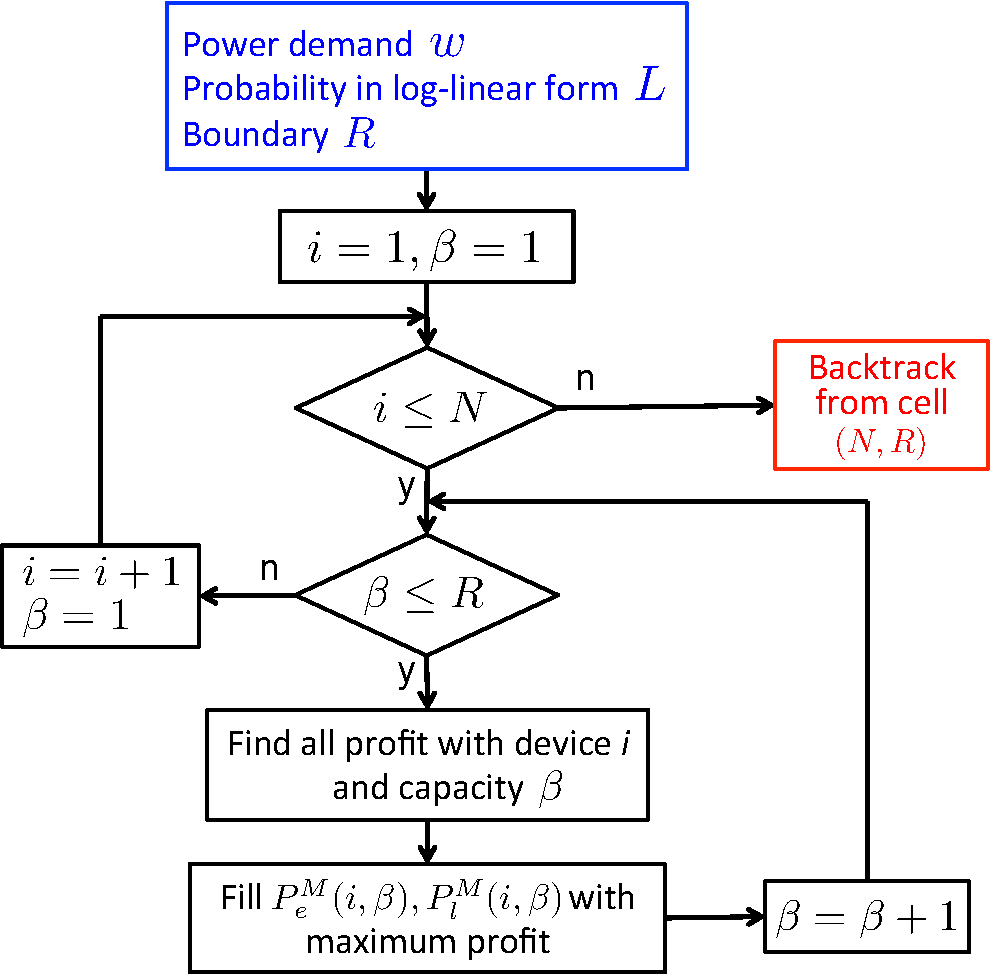
\includegraphics[width=0.6\textwidth]{./chapters/chapter4/images/DPschema.pdf} 
\caption{DP algorithm flowchart. When all entries are filled, the corresponding state vector is obtained by backtracking through the profit tables from the last cell (optimal value).} 
\label{fig:DP1} 
\end{figure}

\begin{algorithm}
\caption{Entry calculation for profit tables in case of multi-state devices.}
\label{algo3}
\begin{algorithmic}[1]
\Ensure $P^M_e(i,\beta),P^M_l(i,\beta)$
\State $Sol(i,\beta) = 0$
\State $a^M_1 = P^M_e(i-1,\beta)$
\State $a^M_2 = P^M_l(i-1,\beta) + \lambda \times l^M_{i0}$
\State $A^M =  \left|a^M_1\right|+a^M_2$
\For{$j=1,\ldots,m_i$}
\If{$w_{ij}\leq \beta$}
\State $b^M_{j1} = P^M_e(i-1,\lfloor \beta-w_{ij}\rfloor)+w_{ij}$
\State $b^M_{j2} = P^M_l(i-1,\lfloor \beta-w_{ij}\rfloor)+\lambda \times l^M_{ij}$
\State $b^M_j = \left|b^M_{j1}\right|+b^M_{j2}$
\Else
\State $b^M_j = +\infty$
\EndIf
\EndFor
\State $k = \min_j{\{b^M_j\}}$; $B^M = b^M_k$
\If{$\min_j{\{w_{ij}\}}\leq \beta$ and $A^M \leq B^M$}
  \State $P^M_e(i,\beta) = a^M_1$
  \State $P^M_l(i,\beta) = a^M_2 $
  \Else
  \State $P^M_e(i,\beta) = b^M_{k1}$
  \State $P^M_l(i,\beta) = b^M_{k2}$
  \State $Sol(i,\beta) = k$
\EndIf
\end{algorithmic}
\end{algorithm}
In other words, the value of each entry when considering a new device is determined by comparing the obtainable profit in two cases: the device is turned off, with profit $A^M$ and the device is operating at a state satisfying the capacity $\beta$, with profit $B^M$.
The initial conditions of the profit tables are
\begin{eqnarray*}
P^M_e(0,\beta) &=& -x,\beta=0,\ldots,R \\
P^M_l(0,\beta)&=&0,\beta = 0,\ldots,R\\
P^M_e(i,0) &=& -x,i=1,\ldots,N\\
P^M_l(i,0)&=&\sum_{j=1}^i{l^M_{j0}},i=1,\ldots,N.
\end{eqnarray*}

To get the state of each device, a backtracking procedure is also constructed as illustrated in Algorithm~\ref{algo4}, in which an additional table $Sol$ with the same size as the profit tables is used to mark the state of devices corresponding to each cell of profit tables.

\begin{algorithm}
\caption{Backtracking algorithm in case of multi-state devices.}
\label{algo4}
\begin{algorithmic}[1]
\Ensure State indicator vector $\mathbf{s} = \{s_1,\ldots,s_N\}$
\State $i = N$ 
\State $\beta =  R$
\While{$i > 0$ and $\beta>0$}
\If{$Sol(i,\beta)>0$}
\State $k = Sol(i,\beta)$
\State $s_i = k$
\State $\beta = \beta-\lceil w_{ik} \rceil $
\State $i = i-1$
\Else
\State $s_i=0$\; $i = i-1$
\EndIf
\EndWhile
\end{algorithmic}
\end{algorithm}

Figure~\ref{fig:DP1} illustrates the flowchart of the proposed DP algorithm in the general case with multi-state devices. Meanwhile, Table~\ref{table:DP2} shows the profit tables relating to the DP algorithm for three multi-state devices with the individual power demand $w_{11}=2$, $(w_{21},w_{22})=(1,4)$, $(w_{31},w_{32}) = (3,5)$ and the respective operating probability $p_{11} = 0.8$, $(p_{21},p_{22}) = (0.7,0.2)$, $(p_{31},p_{32}) = (0.6,0.2)$. The aggregate power consumption $x$ in this example is equal to 6 with standard deviation $\epsilon=0$ and the respective total power boundary $R = \lceil x+\epsilon \rceil = 6$. The regularization parameter $P$ is set to be of $10$. Applying the log-linear form to the operating probability, i.e. $l_{ij} = -\log{p_{ij}},i=1,\ldots,3,j=0,\ldots,m_i$, the corresponding results are $(l_{10},l_{11}) = (0.7,0.1)$, $(l_{20},l_{21},l_{22}) = (1, 0.15, 0.7)$, $(l_{30},l_{31},l_{32}) = (0.7,0.22,0.7)$. Each entry of these tables is calculated by Algorithm~\ref{algo3} and the set of operating state of each device is backtracked through the tables from the optimal point, i.e. $(i,\beta) = (N,R)$, by applying Algorithm~\ref{algo4} is then $\mathbf{s} = (1,1,1)$. This result means that all three devices are operating at the first power state. This determination also satisfies the requirement on the least absolute error on the power consumption and the maximum coincidence operating probability. Presenting vector $\mathbf{s}$ as in Eq.~\ref{eqSS12}, we have $\mathbf{s} = \{1,1,0,1,0\}$.
\begin{table}
\caption{Running example of DP in SmartSense for multi-state devices}\label{table:DP2}
\begin{center}
\begin{tabular}{|c|c|c|c|c|c|c|c|}
\hline
\multicolumn{8}{|c|}{$P^M_e(i,\beta)$}\\ \hline 
$(i,\beta)$&0&1&2&3&4&5&6\\ \hline
0&-6&-6&-6&-6&-6&-6&-6 \\ \hline
1&-6&-6&-4&-4&-4&-4&-4 \\ \hline
2&-6&-5&-5&-3&-3&-3&-3 \\ \hline
3&-6&-5&-5&-3&-3&-3&0 \\ \hline
\multicolumn{8}{|c|}{$P^M_l(i,\beta)$}\\ \hline 
$(i,\beta)$&0&1&2&3&4&5&6\\ \hline
0&0&0&0&0&0&0&0 \\ \hline
1&7&7&1&1&1&1&1\\ \hline
2&17&8.5&8.5&2.5&2.5&2.5&2.5\\ \hline
3&24&15.5&15.5&9.5&9.5&9.5&4.7\\ \hline
\end{tabular}
\end{center}
\end{table}

